\documentclass{kththesis}

\usepackage{textcomp}
\usepackage{lmodern}
\usepackage{amsmath}
\usepackage{amsfonts}
\usepackage{amssymb}
\usepackage{amsthm}
\usepackage{color}
\usepackage{graphicx}
\usepackage{hyperref}
\usepackage[ruled,vlined]{algorithm2e}
\newtheorem{thm}{Theorem}
\definecolor{gris25}{gray}{0.80}
\newcommand{\encadre}[1]{\fcolorbox{black}{gris25}{\begin{minipage}{1.0\textwidth}\medskip #1 \vspace{0.1pt}\end{minipage}}}
\newtheorem{prop}[thm]{Property}
\newtheorem{lem}[thm]{Lemme}
\newtheorem{cor}[thm]{Corollaire}
\newtheorem{hyp}[thm]{Hypothesis}
\def\N{{\mathbb{N}}}
\def\R{{\mathcal{R}}}
\newcommand\independent{\protect\mathpalette{\protect\independenT}{\perp}}
\def\independenT#1#2{\mathrel{\rlap{$#1#2$}\mkern2mu{#1#2}}}
\renewcommand{\thesection}{\arabic{section}}

\usepackage{csquotes} % Recommended by biblatex
\usepackage[style=ieee,backend=bibtex]{biblatex}
\addbibresource{specifications_ref.bib} % The file containing our references, in BibTeX format

\title{Degree project specification:\\
Estimating the probability of event occurrence}
\author{Alexandre GUINAUDEAU}
\email{alegui@kth.se}
\supervisor{Pawel Herman}
\examiner{Hedvig Kjellstr{\"o}m}
\programme{Master in Computer Science}
\school{School of Electrical Engineering and Computer Science}
%\date{\today}

\tolerance=1600

\begin{document}


\maketitle

%\newpage
%\chapter{Specifications}
\section{Background \& objective}

In complex systems, errors can occur intermittently and in a non-deterministic way, which makes it harder to diagnose real errors among spurious ones. 
In manufacturing for instance, intermittent errors could be due to physical properties, either internal, like bad contacts, or external, e.g. extreme temperatures.
In any case, these errors are often hard to troubleshoot and require close attention. By analogy with \emph{flaky tests} in computer science, we will also refer to these as \emph{flaky errors}.\\

Non-deterministic errors are often considered as unreliable and therefore discarded, which creates an important risk of ignoring a real error. On the other hand, troubleshooting each occurrence of a flaky error is very time-consuming and is not always an option. Therefore, it is critical to detect when flaky errors occur at an unexpected rate and to pinpoint when the rate of failure is likely to have evolved. This enables engineers to understand which elements have an impact on the error. In computer science, the usual workaround for flaky tests is to re-run tests that failed a certain number of times until they pass. In other fields, this is not always possible as errors are triggered in a production environment.\\

In this thesis, we intend to estimate the underlying probability of occurrence of an error.
We assume its distribution to be piecewise
stationary. This corresponds to the fact that the probability of
occurrence changes when a part breaks, wears out, or is repaired. Given this assumption, estimating the underlying probability of occurrence is
equivalent to finding its change points.

%In manufacturing plants, aircrafts, electronic intensive care units or data centers, sensors continuously monitor many parameters of the environment  \cite{chambrin1999, bobkoff2015, zhang2014}.
%The data generated by these sensors is then processed to optimize the way the system works, or to diagnose failures once they occurred.
%These systems can have hundreds or thousands of sensors with sub-second sampling.
%With this amount of data, diagnosing failures requires an efficient processing of the data.\\
%
%Finding data that is associated with failures is critical to understand the circumstances of the incident and troubleshoot it. 
%In aircrafts, tens of thousands of sensors monitor various systems to anticipate parts failure and alert pilots of anomalies \cite{bobkoff2015}.
%In data centers, monitoring telemetry data in real time can help understanding past failures and prevent downtime \cite{zhang2014}. 
%
%Usually, providing the system engineer with a limited list of sensors that seem to have some correlation with the failure is very valuable to enable them to quickly troubleshoot the problem.
%Once the engineers know where to look, they are able to understand what happened by diving into the specific environment parameters. 
%Therefore, in this thesis, we do not intend to establish whether one time series is the cause of the other, nor whether there is a positive or linear correlation between them. 
%We only focus on defining a metric that indicates whether the knowledge of one times series can improve the understanding of the other one. \\
%
%In this thesis, we will use the term \emph{association} to refer to the dependency between two time series, as \emph{correlation} is defined for numerical data only.

\section{Interest and assignment}

Given a sequence of events, we intend to detect changes in the probability of occurrence. This has two main interests:

\begin{itemize}
\item Alert when events start occurring more frequently.
\item Troubleshoot errors by pinpointing when the probability of occurrence changed.
\end{itemize}

For instance, in the case of intermittent errors due to bad contact, the detection of change in frequency could enable users to understand that high vibrations triggered the bad contact, and that some specific maintenance work fixed it.

%The main difficulty to find relevant data correlated to triggered events is the heterogeneity of the data: it can be continuous data (for instance measures of environment parameters such as a pressure or a temperature), categorical data (for instance the part that is installed on a machine) or events (for instance when an operation is triggered).
%Some metrics measure association for numerical data, for instance the Pearson coefficient on normalized data \parencite{rodgers1988}, some for categorical data, for instance the J-measure \parencite{goodman1998, smyth1992}. However, none of these generalizes to associating numerical and categorical data with event data.
%
%Tan \parencite{tan2004} compared association metric for binary data on different sets to show they were not equivalent.
%In a similar way, we want to define the expected behavior of association metrics on event, categorical and continuous data and compare existing metrics to define one that matches our expectations.

\section{Objective}

The desired outcome of the degree project is to detect change points in the probability of occurrence of events.
According to \parencite{baigneres2004}, two binomial distributions $Bin(n, p)$ and $Bin(n, p+\varepsilon)$ (where $n$ is the number of observations, and $p \gg \varepsilon$ the probability of occurrence of the event) can be distinguished after 
$$n \sim \dfrac{K}{\varepsilon^2}$$
observations, for some $K$ independent of $\varepsilon$.
So a change in probability of $0.1$ should be detected within the order of $n \sim 100$ observations.

\section{Research question \& method}

\textbf{What is the sensitivity of detection of changes in the frequency of event occurrence? In other words, given a target level of confidence, what is the minimum change in the frequency that can be identified, and what delay is necessary to reliably identify this change?}

%How precisely and how quickly can change points in frequency be detected?
%How big a change in the frequency of occurrence are we able to detect, and how many observations after the change are required to guarantee that the frequency has changed with high confidence?

\medskip

%We will generate data, with examples based on simple probability rules to understand how correlation metrics work and how they can be generalized. 
%Then we will use notional data from open source examples to confirm the hypothesis scale to real-life examples.
% This idea is inspired by Microsoft research's incident diagnosis \parencite{zhang2014}, who monitor statistics on computers such as CPU or memory usage.
%We will compare common metrics -- Pearson, Spearman, Kendall coefficients, J-measure, Mutual information -- that are usually applied to a specific type of data, and try to generalize their definition to continuous, categorical and event data.

% Given time-series of environment parameters, that may be of various nature, how can we define metrics that measure the correlation in an accurate way?

\paragraph*{Examination method \& expected scientific results}

First, we will generate sequences of probabilities of occurrence in a \emph{realistic} way (See \ref{part-lifetime}), and derive events based on those probabilities.
Then, we will try to estimate the underlying probabilities based on the events.
Once this is set up, define a metric to measure the error in the estimation of the underlying sequence of probabilities, and compare different candidate models to find the one that performs best.

Depending on the complexity of the data, we will either use the mathematical definition or approximate it using Monte Carlo methods to evaluate the performance of models.

\medskip

As we will generate the data, it is important to clearly define the assumptions.
Otherwise, the results will be biased by the way we generated the data and will not correctly evaluate the models.
We will generate probabilities of occurrences that either change abruptly, for instance when a part breaks, or that slowly increase, to model the natural deterioration of a part (as explained in \ref{part-lifetime}).


%We will study the properties of metric spaces where the association between heterogeneous time series can be measured and provide an intuitive interpretation.
%
%We will define elementary properties that a good metric should fulfill, and define the expected behavior for simple examples of continuous and categorical data. 
%Models that fulfill these simple rules the best are the ones that measure \emph{association} best.
%
%To compare models, we will simulate time series that are related, as well as time series that are independent, and check whether related time series have higher score than independent ones.
%For synthetic data, we will either use the mathematical definition or Monte-Carlo methods to confirm the validity of the model.

%Finally, we will rank more complex time series based on their association to confirm that highly-associated series have the expected behavior on more complex data.

\paragraph*{Expected scientific results}

The hypothesis being tested is that we are able to detect \emph{significant} changes in probability of occurrence, \emph{shortly} after the change. 
The only parameter of our model should be the target level of confidence (for instance $99\%$). Performing maintenance is usually very expensive as it often requires to replace a part. Therefore, we only want to trigger an alert if we have sufficiently high  confidence that a change in the frequency actually occurred.
%We want to define as few parameters as possible, such as a confidence threshold for the null hypothesis, or the transition probability for the Hidden Markov Model.

Given this, we want to measure:

\begin{itemize}

\item the \emph{sensitivity} of the detection: the minimal increase or decrease in the frequency of occurrence that we are able to detect
\item the \emph{delay} of the detection: the minimal number of observations after a change in frequency  required to detect a change

\end{itemize}


%We will first study usual correlation metrics, and generalize their definition to categorical, event and continuous time-series.
%We expect to be able to determine which metrics are the most suited to define association.

%Finally, we will see whether these metrics are comparable, in other words if it is possible to decide if a categorical time series is more associated to the continuous time series than the events one. This would not be compulsory to solve the problem of incident diagnosis, as it would already be very valuable to find the time series candidates for each type.

\section{Evaluation}

To measure the accuracy of our estimations, we can use the $\mathcal{L}_2$ score to measure the error with the true underlying distribution. We will also measure the error in the detection of a change point, to determine whether we are able to pinpoint the factor that triggered the change.

\paragraph*{News value}


In complex systems, it may be too time-consuming to monitor all the errors that occur. in that case, unusual errors are carefully troubleshooted, but intermittent and non-deterministic errors can end up being ignored. In that case, being able to flag when an error occurs more frequently than usual can be vital. Indicating precisely when the frequency increased significantly is also very useful to quickly understand the reason for this increase in frequency and troubleshoot the error.


%Automatically finding associated sensor time series would be very valuable for all of the systems described above to troubleshoot failures faster and anticipate them. 
%It could be applied to any system that has a logging system generating frequent debug messages and a few error events independently.
%Microsoft researched suggested a solution to correlate continuous and event time series \parencite{zhang2014} but focused more on the temporal correlation - so the causal correlation - rather than the actual association between timeseries. For non-stationary time series, we assume they have been transformed to be stationary - or more exactly, we will show some ways to transform stationary timeseries to stationary ones.

\section{Pilot study}

% My thesis is motivated by a real-world application of incident diagnosis.

\paragraph{Generating events}
\label{part-lifetime}

To generate our data, we will simulate part failures that lead to an increased probability of triggered events. Interestingly, the lifetime of organisms, devices, structures, materials in both biological and engineering sciences have very similar behaviors. 
For example, business mortality \parencite{lomax1954}, failures in the air-conditioning equipment of aircrafts or in semiconductors \parencite{proschan1963} and integrated circuit modules \cite{saunders1983} all have similar behaviors. 
These can be modeled with a mixture of exponential or Weibull-Lomax distributions. In particular, the Weibull distribution \parencite{weibull1951} is the most widely used to model the lifetime of parts \parencite{anderson2005}, as it has a limited number of parameters which can easily be interpreted, and captures both the \emph{infant mortality} of defective parts and the exponential distribution of events that occur independently at a constant average rate, for normal parts. The two parameters are used to reflect these two elements, the defects in the material and the average rate of failure.


\paragraph{Detection of probability change-points}

The detection of a change point can be formulated as a null hypothesis that determines whether all events were drawn from the same binomial distribution \parencite{wasserman2004}.
To generalize this to multiple change points, we could use a sliding window. However, this is often unstable because the change point detection is performed on small regions, and therefore isn't always statistically significant \parencite{esteller2001, harchaoui2010}.
Therefore, we will also explore binary segmentation or dynamic programming to generalize our algorithm to sequences of events with multiple change points \parencite{jackson2005}, while still running in linear time \parencite{killick2012}.


Another lead could be to use Hidden Markov Models \parencite{baum1966}, which seems well-adapted to our use case, as we are trying to guess the hidden probability state that was used to generate the events. Chis and Harrison \parencite{chis2015} suggest a solution to adapt the model to online problems by estimating its updated parameters. This can be used to avoid recomputing the hidden state with new values.

%The most common metric to measure correlation is the \emph{Pearson} coefficient. It can easily be interpreted and visualized \parencite{rodgers1988}, and often gives very good results. However, in some case, it can be misleading, especially because it only captures linear correlations and because it assumes normal distribution of the input parameters.
%
%In this case, the \emph{Spearman} coefficient is more robust (although less efficient), as it only compares ranks between elements, and therefore captures monotonic correlations, even if there are not linear. The \emph{Kendall} coefficient is very similar as it also uses the rank of elements to compare them, it is less efficient but more robust. It is also much easier to interpret, as it captures the percentage of elements positively correlated \parencite{valz1994, xu2010}. These correlation metrics are probably more adapted to our problem for numerical data as they capture non-linear correlations, but may be harder to generalize because their definition is not as simple as Pearson's.
%
%\newpage
%
%\paragraph{Association metrics}
%
%All these usual correlation metrics apply to numerical data, and cannot therefore be used for categorical data. In this case, a metric that often works well is the J-measure \parencite{smyth1992, goodman1998}, which is based on the concept of entropy in information theory. For binary data, it is possible to transform the data to make most association measures equivalent \parencite{tan2004}. This is not as clear for more complex data, and requires to clearly define the concept of association for categorical and continuous data as well.
%
%However, it is not clear if this measure can be compared to the previous ones when the data is both numerical and categorical - for instance when it is binary. In \parencite{tan2004}, P-N Tan et al. compared many existing norms on binary classification, and showed their was a way to normalize the data in order to make all the norms they studied equivalent. Such techniques will be important to pre-process the data accurately and to generalize norms to heterogeneous time series.
%
%\paragraph{Application to heterogeneous data}
%Several tools exist to analyze the correlation between continuous time series \parencite{wu2010}, or between events \parencite{lou2010}, but they do not perform well when it comes to correlating continuous time series and events. However, sensor data is heterogeneous: it can be continuous, discrete, categorical or binary.
%Usual measures of correlation such as the Pearson and Spearman correlation do not perform well on this kind of data \parencite{zhang2014}.
%Therefore, we have to find other ways of defining association. We can also map continuous or categorical time series to event time series - by detecting outliers or change points - and apply existing tools to the transformed data \parencite{stoffer1993, guralnik1999}.

% A lot of work has been done to detect anomalies in continuous time series. Most sensor data - such as Climate \parencite{frankignoul1977}, Intensive Care Units \parencite{chambrin1999} or computer resources \parencite{zhang2014} - has natural frequencies.
% It is therefore possible to find pseudo-periods in the data that facilitate its pre-processing and enable multi-scale analysis \parencite{costa2002}.
% In other words, the time series can be decomposed into scales, in order to detect both local \parencite{knorr1998, ramaswamy2000, angiulli2002} and global anomalies \parencite{breunig2000, shahabi2001}.
% Shahabi et al. even defined a surprise score that enables the comparison of all of these potential outliers, regardless of the scale \parencite{shahabi2000}.


% Finally, a completely different approach to this problem could be to cluster timeseries (for example using the method described in \parencite{keogh2004}), and then find the best candidates within the event's cluster. Time series that are similar to the failure time series are more likely to be correlated. \\


\section{Conditions \& schedule}

%Resources needed to solve the problem consist in the access to the data and the infrastructure to store and process it.


\paragraph*{Limitations}

We will only work on generated data and therefore we will not confirm the validity of the results on real world data.

%The data we will use to compare metrics will be generated. We will explain how real data could be cleaned, but will not go into details, as this largely depends on what the data represents.
%We do not try to determine whether associated time series are a cause of one another, but simply that the knowledge of one of them can help understanding the other one.

\paragraph*{Collaboration with principal supervisor}

My supervisor will mostly contribute in general thesis and problem definition.

\begin{figure}[ht]
	\centering
  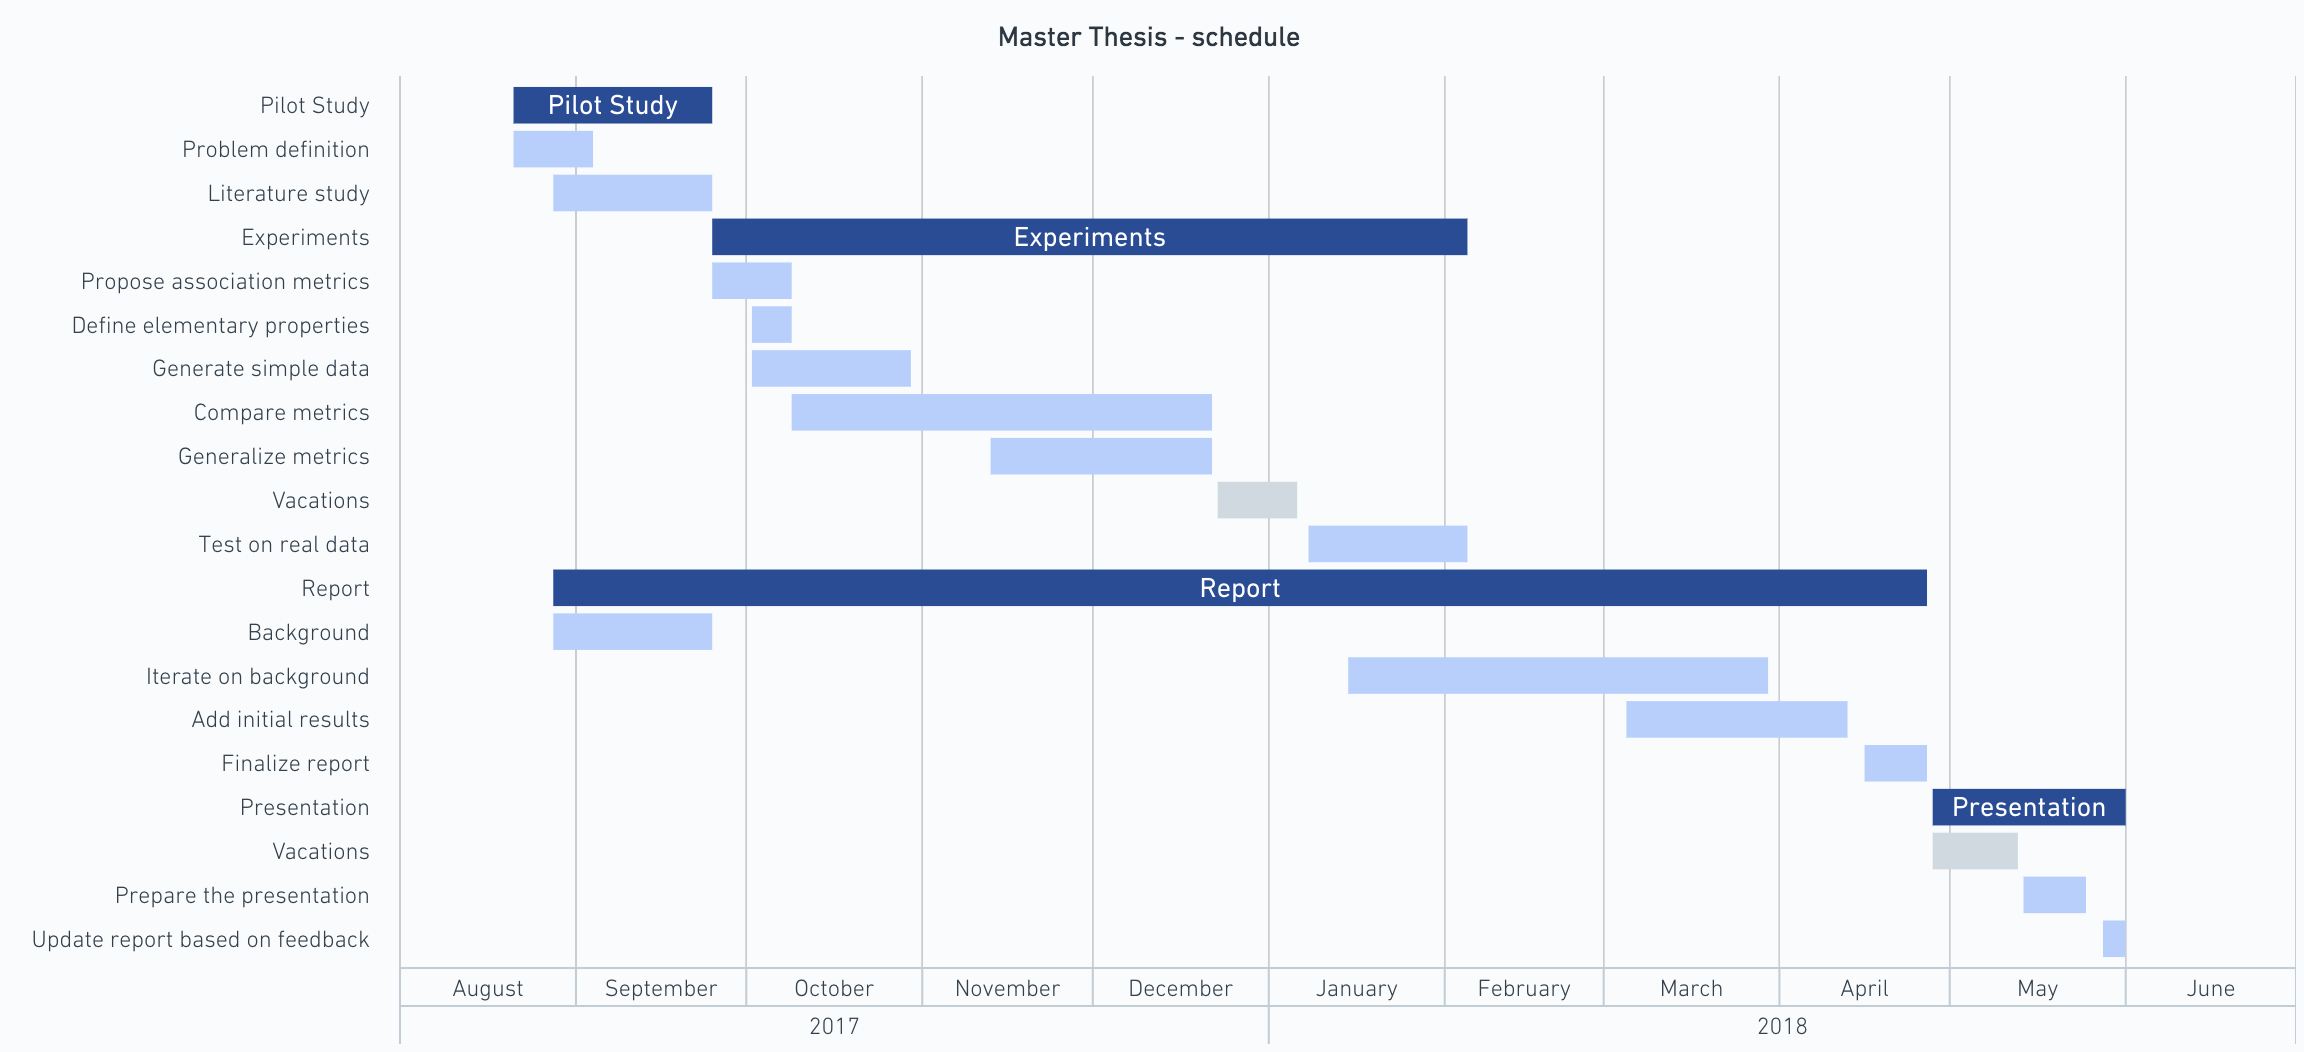
\includegraphics[width=0.95\textheight, angle=90]{gantt.png}
	\caption{Schedule}
	\label{fig}
\end{figure}

\clearpage

\printbibliography[heading=bibintoc]

% \tableofcontents

%
%\begin{thebibliography}{9}
%% Climate
%\bibitem{frankignoul1977}
%Claude Frankignoul, Klaus Hasselmann (1977) \\
%\textit{Stochastic climate models, Part II - Application to sea-surface temperature anomalies and thermocline variability},
%Tellus, 29:4, 289-305\\
%% \url{https://doi.org/10.3402/tellusa.v29i4.11362}
%
%% Categorical Time series
%\bibitem{stoffer1993}
%David S. Stoffer, David E. Tyler, Andrew J. McDougall (1993)\\
%\textit{Spectral Analysis for Categorical Time Series: Scaling and the Spectral Envelope},
%Biometrika Vol. 80, No. 3, pp. 611-622\\
%% \url{https://www.researchgate.net/profile/David_Tyler2/publication/239726763_Spectral_Analysis_for_Categorical_Time_Series_Scaling_and_the_Spectral_Envelope/links/0046352d842c990d8d000000.pdf}
%
%% distance-based outliers
%\bibitem{rodgers1988}
%Joseph Lee Rodgers and W. Alan Nicewander (1987)\\
%\textit{Thirteen Ways to Look at the Correlation Coefficient}, pp 59-66
%Download citation  https://doi.org/10.1080/00031305.1988.10475524
%
%\bibitem{smyth1992}
%Smyth, P. and Goodman, R.M. (1992)\\
%\emph{An Information Theoretic Approach to Rule Induction from Databases}, IEEE Transactions on Knowledge and Data Engineering, 4 (Aug. 1992), 301-316
%
%\bibitem{valz1994}
%Valz P.D. \& Thompson M.E. (1994) \\
%\textit{Exact inference for Kendall's
%S and Spearman's rho}, Journal of Computational and
%Graphical Statistics 3: 459-472.
%
%\bibitem{knorr1998}
%E. M. Knorr and R. T. Ng. (1998)\\
%\textit{Algorithms for Mining Distance-Based Outliers}, In Proceedings of the 24th
%International Conference on Very Large Databases (VLDB), pages 392-403, 1998.\\
%% \url{http://www.vldb.org/conf/1998/p392.pdf}
%
%\bibitem{goodman1998}
%Goodman, R.M. and Smyth, P. (1998)\\
%\emph{An information-theoretic model for rule-based expert systems}, Int. Symposium in Information Theory, Kobe, Japan, 1988
%
%% Iterative partitioning of time segments to detect change points
%\bibitem{guralnik1999}
%Valery Guralnik, Jaideep Srivastava (1999)\\
%\textit{Event Detection from Time Series Data}, In Proceedings of the Fifth ACM SIGKDD International Conference on Knowledge Discovery and Data Mining (KDD'99), pp. 33-42, August 15-18, 1999, San Diego, CA, USA. \\
%% \url{http://dmr.cs.umn.edu/Papers/P1999_6.pdf}
%
%% Different kinds of sensors:
%% Intensive Care Unit => alerts based on hardcoded thresholds
%\bibitem{chambrin1999}
%M.-C. Chambrin, P. Ravaux, D. Calvelo-Aros, A. Jaborska, C. Chopin, B. Boniface (1999)\\
%\textit{Multicentric study of monitoring alarms in the adult intensive care unit (ICU): a descriptive analysis},
%Intensive Care Medicine, Volume 25, Issue 12, pp 1360-1366\\
%% \url{https://doi.org/10.1007/s001340051082}
%
%\bibitem{ramaswamy2000}
%S. Ramaswamy, R. Rastogi, and K. Shim. (2000)\\
%\textit{Efficient algorithms for mining outliers from large data sets}, In
%SIGMOD '00: Proceedings of the 2000 ACM SIGMOD international conference on Management of
%data, pages 427-438, 2000.
%% \url{https://dl.acm.org/citation.cfm?id=335437&dl=ACM&coll=DL&CFID=841695128&CFTOKEN=52089307}
%
%\bibitem{breunig2000}
%M. M. Breunig, H. Kriegel, R. T. Ng, and J. Sander (2000)\\
%\textit{LOF: Identifying density-based local outlier}
%In Proceedings of the ACM SIGMOD International Conference on Management of Data, pages 93-104, 2000\\
%% \url{http://www.dbs.ifi.lmu.de/Publikationen/Papers/LOF.pdf}
%
%% \bibitem{shahabi2000}
%% C. Shahabi, X. Tian, and W. Zhao. TSA-tree (2000)\\
%% \textit{A wavelet-based approach to improve the efficiency of multilevel surprise and trend queries on time-series data},
%% In Statistical and Scientific Database Management, pages 55-68, 2000.\\
%% \url{https://infolab.usc.edu/DocsDemos/pakdd01.pdf}
%
%\bibitem{shahabi2001}
%C.Shahabi, S. Chung, M.Safar and G.Ha jj (2001)\\
%\textit{2D TSA-tree: A Wavelet-Based Approach to Improve the Efficiency of Multi-Level Spatial Data Mining},
%Technical Report 01-740, Department of Computer Science, University of Southern California. (2001)\\
%% \url{https://pdfs.semanticscholar.org/39c5/5ee09a2c49e736de730e2cc7cc61f789ace1.pdf}
%% Tree splitting each signal in 2, a low-pass and a high-pass signal – Detect global outlier regions and local outliers within regions
%
%\bibitem{angiulli2002}
%F. Angiulli and C. Pizzuti. (2002)\\
%\textit{Fast outlier detection in high dimensional spaces},In PKDD '02: Proceedings
%of the 6th European Conference on Principles of Data Mining and Knowledge Discovery, pages 15-26,
%2002
%% \url{https://link.springer.com/chapter/10.1007/3-540-45681-3_2}
%
%% Multiscale timeseries + multiscale entropy (Computed for several down-samples of the original timeseries)
%\bibitem{costa2002}
%Costa M, Goldberger AL, Peng CK (2002)\\
%\textit{Multiscale entropy analysis of complex physiologic time series},
%Phys Rev Lett 2002, 89: 068102. 10.1103/PhysRevLett.89.068102\\
%% \url{https://dbiom.org/files/publications/Peng_MultiscaleEntropyAnalysisComplexPhysiologicTimeSeries.pdf}
%
%\bibitem{tan2004}
%Pang-Ning Tan*, Vipin Kumar, Jaideep Srivastava (2004)\\
%\textit{Selecting the right objective measure for association analysis}
%
%% % Parameter-free clustering of similar time series
%% \bibitem{keogh2004}
%% Keogh, E., Lonardi, S., Ratanamahatana, C. (2004)\\
%% \textit{Towards Parameter-Free Data Mining},
%% In proceedings of the 10th ACM SIGKDD International Conference on Knowledge Discovery and Data Mining.\\
%% \url{http://www.cs.ucr.edu/~eamonn/SIGKDD_2004_long.pdf}
%
%\bibitem{rebbapragada2009}
%Umaa Rebbapragada, Pavlos Protopapas, Carla E. Brodley, Charles Alcock (2009)\\
%\textit{Finding anomalous periodic time series}
%Machine Learning, v.74 n.3, p.281-313, March 2009. doi: 10.1007/s10994-008-5093-3\\
%% \url{https://arxiv.org/pdf/0905.3428.pdf}
%
%\bibitem{xu2010}
%Xu Weichao, Yunhe Hou, Hung Y. S. \& Yuexian Zou (2010)\\
%\textit{Comparison of Spearman's rho and Kendall's tau in normal and contaminated normal models}, Manuscript submitted to IEEE Transactions on Information Theory\\
%% \url{http://arxiv.org/PS_cache/arxiv/pdf/1011/1011.2009v1.pdf}
%
%\bibitem{lou2010}
% J.-G. Lou, Q. Fu, Y. Wang, and J. Li (2010)\\
%\textit{Mining dependency in distributed systems through unstructured logs analysis}, SIGOPS Operating Systems Review, 41(1):91-96, 2010.
%
%\bibitem{wu2010}
%D. Wu, Y. Ke, J. X. Yu, S. Y. Philip, and L. Chen (2010)\\
%\textit{Detecting leaders from correlated time series}, In Database Systems for Advanced Applications, pages 352-367. Springer.
%
%\bibitem{zhang2014}
%Zhang, Dongmei and Lou, Jian-Guang and Ding, Justin and Fu, Qiang and Lin, Qingwei (2014)\\
%\textit{Correlating Events with Time Series for Incident Diagnosis},
%SigKDD'14, July 2014\\
%% \url{https://www.microsoft.com/en-us/research/publication/correlating-events-time-series-zhang2014-2/}
%
%
% % Down-sampling time-series and measuring information lost
% \bibitem{cui2015}
% H. Cui, K. Keeton, I. Roy, K. Viswanathan, and G. R. Ganger (2015)\\
% \textit{Using data transformations for low-latency time series analysis},
% In Proceedings of the Sixth ACM Symposium on Cloud Computing, pages 395-407. ACM, 2015\\
% \url{https://www.labs.hpe.com/techreports/2015/HPL-2015-74.pdf}
%
%\end{thebibliography}


% Online estimation biology
% https://link.springer.com/article/10.1007/BF02345755

\end{document}
